\documentclass{article}\usepackage[]{graphicx}\usepackage[]{color}
%% maxwidth is the original width if it is less than linewidth
%% otherwise use linewidth (to make sure the graphics do not exceed the margin)
\makeatletter
\def\maxwidth{ %
  \ifdim\Gin@nat@width>\linewidth
    \linewidth
  \else
    \Gin@nat@width
  \fi
}
\makeatother

\definecolor{fgcolor}{rgb}{0.345, 0.345, 0.345}
\newcommand{\hlnum}[1]{\textcolor[rgb]{0.686,0.059,0.569}{#1}}%
\newcommand{\hlstr}[1]{\textcolor[rgb]{0.192,0.494,0.8}{#1}}%
\newcommand{\hlcom}[1]{\textcolor[rgb]{0.678,0.584,0.686}{\textit{#1}}}%
\newcommand{\hlopt}[1]{\textcolor[rgb]{0,0,0}{#1}}%
\newcommand{\hlstd}[1]{\textcolor[rgb]{0.345,0.345,0.345}{#1}}%
\newcommand{\hlkwa}[1]{\textcolor[rgb]{0.161,0.373,0.58}{\textbf{#1}}}%
\newcommand{\hlkwb}[1]{\textcolor[rgb]{0.69,0.353,0.396}{#1}}%
\newcommand{\hlkwc}[1]{\textcolor[rgb]{0.333,0.667,0.333}{#1}}%
\newcommand{\hlkwd}[1]{\textcolor[rgb]{0.737,0.353,0.396}{\textbf{#1}}}%

\usepackage{framed}
\makeatletter
\newenvironment{kframe}{%
 \def\at@end@of@kframe{}%
 \ifinner\ifhmode%
  \def\at@end@of@kframe{\end{minipage}}%
  \begin{minipage}{\columnwidth}%
 \fi\fi%
 \def\FrameCommand##1{\hskip\@totalleftmargin \hskip-\fboxsep
 \colorbox{shadecolor}{##1}\hskip-\fboxsep
     % There is no \\@totalrightmargin, so:
     \hskip-\linewidth \hskip-\@totalleftmargin \hskip\columnwidth}%
 \MakeFramed {\advance\hsize-\width
   \@totalleftmargin\z@ \linewidth\hsize
   \@setminipage}}%
 {\par\unskip\endMakeFramed%
 \at@end@of@kframe}
\makeatother

\definecolor{shadecolor}{rgb}{.97, .97, .97}
\definecolor{messagecolor}{rgb}{0, 0, 0}
\definecolor{warningcolor}{rgb}{1, 0, 1}
\definecolor{errorcolor}{rgb}{1, 0, 0}
\newenvironment{knitrout}{}{} % an empty environment to be redefined in TeX

\usepackage{alltt}
% \VignetteIndexEntry{\texttt{bnstruct}: an R package for Bayesian Network Structure Learning}
% \VignettePackage{bnstruct}
% \VignetteKeywords{Documentation}
%\VignetteEngine{knitr::knitr}
\usepackage{url}
\usepackage[numbers]{natbib}\citeindextrue

\newcommand{\Rfunction}[1]{{\texttt{#1}}}
\newcommand{\Robject}[1]{{\texttt{#1}}}
\newcommand{\Rpackage}[1]{{\texttt{#1}}}
\newcommand{\Rmethod}[1]{{\texttt{#1}}}
\newcommand{\Rfunarg}[1]{{\texttt{#1}}}
\newcommand{\Rclass}[1]{{\textit{#1}}}
\IfFileExists{upquote.sty}{\usepackage{upquote}}{}
\begin{document}




\title{\texttt{bnstruct}: an R package for Bayesian Network Structure Learning with missing data}
\author{Francesco Sambo, Alberto Franzin}
\maketitle



\section{Introduction}
Bayesian Networks (\citet{pearl1988probabilistic}) are a powerful tool for probabilistic inference among a set
of variables, modeled using a directed acyclic graph. However, one often does not
have the network, but only a set of observations, and wants to reconstruct the
network that generated the data. The \Rpackage{bnstruct} package provides objects and methods for
learning the structure and parameters of the network in various situations, such as
in presence of missing data, for which it is possible to perform \textit{imputation}
(guessing the missing values, by looking at the data). The package also contains methods
for learning using the Bootstrap technique.
Finally, \Rpackage{bnstruct}, has a set of additional tools to use Bayesian Networks, such as methods to perform
belief propagation.

In particular, the absence of some observations in the dataset is a very common situation in real-life
applications such as biology or medicine, but very few software around is devoted to address these problems.
\Rpackage{bnstruct} is developed mainly with the purpose of filling this void.

This document is intended to show some examples of how \Rpackage{bnstruct} can be used
to learn and use Bayesian Networks. First we describe how to manage data sets,
how to use them to discover a Bayesian Network, and finally how to perform some
operations on a network. Complete reference for classes and methods can be found in the package documentation.

\subsection{Overview}
We provide here some general informations about the context for understanding
and using properly this document. A more thorough introduction to the topic can be found for example in
\citet{koller2009probabilistic}.

\subsubsection{The data}
A \emph{dataset} is a collection of rows, each of which is composed by the same number
of values. Each value corresponds to an observation of a \emph{variable}, which is a feature,
an event or an entity considered significant and therefore measured. In a Bayesian Network,
each variable is associated to a node. The number of variables is the \emph{size} of the
network. Each variable has a certain range of values it can take. If the variable can take
any possible value in its range, it is called a \emph{continuous} variable; otherwise,
if a variable can only take some values in its range, it is a \emph{discrete} variable.
The number of values a variable can take is called its \emph{cardinality}.
A continuous variable has infinite cardinality; however, in order to deal with it,
we have to restrict its domain to a smaller set of values, in order to be able to
treat it as a discrete variable; this process is called \emph{quantization}, the
number of values it can take is called the number of \emph{levels} of the quantization step,
and we will therefore call the cardinality of a continuous variable the number of its
quantization levels, with a little abuse of terminology.

In many real-life applications and contexts, it often happens that some observations in
the dataset we are studying are absent, for many reasons. In this case, one may want to
``guess'' a reasonable (according to the other observations) value that would have been
present in the dataset, if the observations was successful. This inference task is
called \emph{imputation}. In this case, the dataset with the ``holes filled''
is called the \emph{imputed dataset}, while the original dataset with missing values is
referred to as the \emph{raw dataset}.
In section \ref{sec:imputation} we show how to perform imputation in \Rpackage{bnstruct}.

Another common operation on data is the employment of resampling techniques in order
to estimate properties of a distribution from an approximate one. This usually allows
to have more confidence in the results. We implement the \emph{bootstrap} technique (\citet{efron1994introduction}),
and provide it to generate samples of a dataset, with the chance of using it on both raw and imputed data.

\subsubsection{Bayesian Networks}
After introducing the data, we are now ready to talk about \emph{Bayesian Networks}. A Bayesian Network
(hereafter sometimes simply \emph{network}, \emph{net} or \emph{BN} for brevity) is a probabilistic graphical model that encodes
the conditional dependency relationships of a set of variables using a Directed Acyclic Graph (DAG).
Each node of the graph represents one variable of the dataset; we will therefore interchange
the terms \emph{node} and \emph{variable} when no confusion arises. The set of directed edges
connecting the nodes forms the \emph{structure} of the network, while the set of conditional
probabilities associated with each variable forms the set of \emph{parameters} of the net.

The DAG is represented as an \textit{adjacency matrix}, a $n\times n$ matrix, where $n$ is the number of nodes,
whose cells of indices $(i,j)$ take value $1$ if there is an edge going from node $i$ to node $j$,
and $0$ otherwise.

The problems of learning the structure and the parameters of a network from data define the
\emph{structure learning} and \emph{parameter learning} tasks, respectively. 

Given a dataset of observations, the structure learning problem is the problem of finding the DAG of a
network that may have generated the data. Several algorithms have been proposed fot this problem, but
a complete search is doable only for networks with no more than 20-30 nodes. For larger networks, several
heuristic strategies exist.

The subsequent problem of parameter learning, instead, aims to discover the conditional probabilities
that relate the variables, given the dataset of observations and the structure of the network.

In addition to structure learning, sometimes it is of interest to estimate a level of the confidence 
on the presence of an edge in the network. This is what happens when we apply bootstrap to the problem
of structure learning. The result is not a DAG, but a different entity that we call \emph{weighted partially DAG},
which is an adjacency matrix whose cells of indices $(i,j)$ take the number of times that an edge going from node $i$
to node $j$ appear in the network obtained from each bootstrap sample.

As the graph obtained when performing structure learning with bootstrap represents a measure of the confidence
on the presence of each edge in the original network, and not a binary response on the presence of the edge,
the graph is likely to contain undirected edges or cycles.

As the structure learnt is not a DAG but a measure of confidence, it cannot be used to learn conditional probabilities.
Therefore, parameter learning is not defined in case of network learning with bootstrap.

One of the most relevant operations that can be performed with a Bayesian Network is to perform \emph{inference} with it.
Inference is the operations that, given a set of observed variables, computes the probabilities of the remaining variables
updated according to the new knowledge. Inference answers questions like ``How does the probability for variable
$Y$ change, given that variable $X$ is taking value $x\prime$?''.

\section{Installation}
The latest stable version of the package is available on CRAN \url{https://cran.r-project.org},
and can therefore be installed from an R session using
\begin{knitrout}
\definecolor{shadecolor}{rgb}{0.969, 0.969, 0.969}\color{fgcolor}\begin{kframe}
\begin{alltt}
\hlstd{> }\hlkwd{install.packages}\hlstd{(}\hlstr{"bnstruct"}\hlstd{)}
\end{alltt}
\end{kframe}
\end{knitrout}

The latest development version of \Rpackage{bnstruct} can be found at \url{http://github.com/sambofra/bnstruct}.

In order to install the package, it suffices to open a shell and run
\begin{knitrout}
\definecolor{shadecolor}{rgb}{0.969, 0.969, 0.969}\color{fgcolor}\begin{kframe}
\begin{alltt}
git clone https://github.com/sambofra/bnstruct.git
cd bnstruct
make install
\end{alltt}
\end{kframe}
\end{knitrout}

\Rpackage{bnstruct} requires R $\geq 2.10$,
and depends on \Rpackage{bitops}, \Rpackage{igraph}, \Rpackage{Matrix} and \Rpackage{methods}.
Package \Rpackage{Rgraphviz} is requested in order to plot graphs, but is not mandatory.


\section{Data sets}
The class that \Rpackage{bnstruct} provides to manage datasets is \Robject{BNDataset}.
It contains all of the data and the informations related to it: raw and imputed data, raw and imputed
bootstrap samples, and variable names and cardinality.

\subsection{Creating a BNDataset}
There are two ways to build a BNDataset: using two files containing respectively header informations
and data, and manually providing the data table and the related header informations
(variable names, cardinality and discreteness).

\begin{knitrout}
\definecolor{shadecolor}{rgb}{0.969, 0.969, 0.969}\color{fgcolor}\begin{kframe}
\begin{alltt}
\hlstd{> }\hlstd{dataset.from.data} \hlkwb{<-} \hlkwd{BNDataset}\hlstd{(}\hlkwc{data} \hlstd{= data,}
\hlstd{+ }                               \hlkwc{discreteness} \hlstd{=} \hlkwd{rep}\hlstd{(}\hlstr{'d'}\hlstd{,}\hlnum{4}\hlstd{),}
\hlstd{+ }                               \hlkwc{variables} \hlstd{=} \hlkwd{c}\hlstd{(}\hlstr{"a"}\hlstd{,} \hlstr{"b"}\hlstd{,} \hlstr{"c"}\hlstd{,} \hlstr{"d"}\hlstd{),}
\hlstd{+ }                               \hlkwc{node.sizes} \hlstd{=} \hlkwd{c}\hlstd{(}\hlnum{4}\hlstd{,}\hlnum{8}\hlstd{,}\hlnum{12}\hlstd{,}\hlnum{16}\hlstd{))}
\hlstd{> }
\hlstd{> }\hlstd{dataset.from.file} \hlkwb{<-} \hlkwd{BNDataset}\hlstd{(}\hlstr{"path/to/data.file"}\hlstd{,}
\hlstd{+ }                               \hlstr{"path/to/header.file"}\hlstd{)}
\end{alltt}
\end{kframe}
\end{knitrout}

The key informations needed are:
\begin{enumerate}
\item the data;
\item the state of variables (discrete or continuous);
\item the names of the variables;
\item the cardinalities of the variables (if discrete), or the number of levels they have to be quantized into
(if continuous). 
\end{enumerate}
Names and cardinalities/leves can be guessed by looking at the data, but it is strongly advised to provide
\textit{all} of the informations, in order to avoid problems later on during the execution.

Data can be provided in form of data.frame or matrix. It can contain NAs. By default, NAs are indicated with '?';
to specify a different character for NAs, it is possible to provide also the \texttt{na.string.symbol} parameter.
The values contained in the data have to be numeric (real for continuous variables, integer for discrete ones).
The default range of values for a discrete variable \texttt{X} is \texttt{[1,|X|]}, with \texttt{|X|} being
the cardinality of \texttt{X}. The same applies for the levels of quantization for continuous variables.
If the value ranges for the data are different from the expected ones, it is possible to specify a different
starting value (for the whole dataset) with the \texttt{starts.from} parameter. E.g. by \texttt{starts.from=0}
we assume that the values of the variables in the dataset have range \texttt{[0,|X|-1]}.
Please keep in mind that the internal representation of Rpackage{bnstruct} starts from 1,
and the original starting values are then lost. 

It is possible to use two files, one for the data and one for the metadata,
instead of providing manually all of the info. 
bnstruct requires the data files to be in a format subsequently described.
The actual data has to be in (a text file containing data in) tabular format, one tuple per row,
with the values for each variable separated by a space or a tab. Values for each variable have to be
numbers, starting from \texttt{1} in case of discrete variables.
Data files can have a first row containing the names of the corresponding variables.

In addition to the data file, a header file containing additional informations can also be provided.
An header file has to be composed by three rows of tab-delimited values:
\begin{enumerate}
\item list of names of the variables, in the same order of the data file;
\item a list of integers representing the cardinality of the variables, in case of discrete variables,
 or the number of levels each variable has to be quantized in, in case of continuous variables;
\item a list that indicates, for each variable, if the variable is continuous
 (\texttt{c} or \texttt{C}), and thus has to be quantized before learning,
 or discrete (\texttt{d} or \texttt{D}).
\end{enumerate}
In case of need of more advanced options when reading a dataset from files, please refer to the
documentation of the \texttt{read.dataset} method. Imputation and bootstrap are also available
as separate routines (\texttt{impute} and \texttt{bootstrap}, respectively).

We provide two sample datasets, one with complete data (the \texttt{Asia} network, \citet*{lauritzen1988local}) and one with missing values
(the \texttt{Child} network, \citet*{spiegelhalter1993bayesian}), in the \texttt{extdata} subfolder;
the user can refer to them as an example. The two datasets have been created with

\begin{knitrout}
\definecolor{shadecolor}{rgb}{0.969, 0.969, 0.969}\color{fgcolor}\begin{kframe}
\begin{alltt}
\hlstd{> }\hlstd{asia} \hlkwb{<-} \hlkwd{BNDataset}\hlstd{(}\hlstr{"asia_10000.data"}\hlstd{,}
\hlstd{+ }                  \hlstr{"asia_10000.header"}\hlstd{,}
\hlstd{+ }                  \hlkwc{starts.from}\hlstd{=}\hlnum{0}\hlstd{)}
\hlstd{> }\hlstd{child} \hlkwb{<-} \hlkwd{BNDataset}\hlstd{(}\hlstr{"Child_data_na_5000.data"}\hlstd{,}
\hlstd{+ }                   \hlstr{"Child_data_na_5000.header"}\hlstd{,}
\hlstd{+ }                   \hlkwc{starts.from}\hlstd{=}\hlnum{0}\hlstd{)}
\end{alltt}
\end{kframe}
\end{knitrout}

and are also available with

\begin{knitrout}
\definecolor{shadecolor}{rgb}{0.969, 0.969, 0.969}\color{fgcolor}\begin{kframe}
\begin{alltt}
\hlstd{> }\hlstd{asia}  \hlkwb{<-} \hlkwd{asia}\hlstd{()}
\hlstd{> }\hlstd{child} \hlkwb{<-} \hlkwd{child}\hlstd{()}
\end{alltt}
\end{kframe}
\end{knitrout}


% \subsection{Importing a dataset}
% The preferred way to create a \Rclass{BNDataset} object is by reading a dataset from a file.
% In order to accomplish this, we provide the \Rmethod{read.dataset} method.
% 
% <<read.dataset,eval=FALSE>>=
% dataset <- BNDataset(name="Example")
% dataset <- read.dataset(dataset,
%                         header.file = "path/to/file.header",
%                         data.file   = "path/to/file.data")
% @
% 
% The sample datasets we provide come with two custom loaders:
% <<sample.datasets>>=
% asia.data  <- asia()
% child.data <- child()
% @
% 
% \subsection{Creating a \Robject{BNDataset} from data}
% Another possible way for creating a \Robject{BNDataset} is to create it from a \Rclass{data.frame} or a \Rclass{matrix}
% and some metadata. This is useful, for example, for instantiating a dataset after the data has already been 
% processed in some way.
% 
% In particular, it is requested to provide the data, in \texttt{data.frame} or \texttt{matrix} form, and three additional
% vectors of informations on the domain: one containing the names of the variables, another one containing values indicating
% the cardinality (for discrete variables) or the quantization domain (for continuous variables) of the variables,
% and the last one containing the status of the variables (\texttt{c} for continuous, \texttt{d} for discrete). Please note that
% all of the metadata are required when choosing this option, and it is also suggested that the slot names
% are specified when passing data and metadata as parameters to the constructor;
% when no dataset name is provided, the slot names are mandatory.
% 
% <<bndataset2,eval=FALSE>>==
% data <- matrix(c(1:16), nrow = 4, ncol = 4)
% dataset <- BNDataset(name = "MyData", data = data,
%                      variables = c("a", "b", "c", "d"),
%                      node.sizes = c(4,8,12,16),
%                      discreteness = rep('d',4))
% @

\subsection{Imputation}\label{sec:imputation}
A dataset may contain various kinds of missing data, namely unobserved variables,
and unobserved values for otherwise observed variables. We currently deal only with this
second kind of missing data. The process of guessing the missing values is called \emph{imputation}.

We provide the \Rmethod{impute} function to perform imputation.
\begin{knitrout}
\definecolor{shadecolor}{rgb}{0.969, 0.969, 0.969}\color{fgcolor}\begin{kframe}
\begin{alltt}
\hlstd{> }\hlstd{dataset} \hlkwb{<-} \hlkwd{BNDataset}\hlstd{(}\hlkwc{data.file}   \hlstd{=} \hlstr{"path/to/file.data"}\hlstd{,}
\hlstd{+ }                     \hlkwc{header.file} \hlstd{=} \hlstr{"path/to/file.header"}\hlstd{)}
\hlstd{> }\hlstd{dataset} \hlkwb{<-} \hlkwd{impute}\hlstd{(dataset)}
\end{alltt}
\end{kframe}
\end{knitrout}

Imputation is accomplished with the k-Nearest Neighbour algorithm. The number of neighbours to be used
can be chosen specifying the \Rfunarg{k.impute} parameter (default is \Rfunarg{k.impute = 10}). Given that
the parameter is highly dataset-dependant, we also include the \Rmethod{tune.knn.impute} function to assist
the user while choosing the best value for \Rfunarg{k}.

\subsection{Bootstrap}
\Robject{BNDataset} objects have also room for bootstrap samples (\citet{efron1994introduction}), i.e. random samples with replacement of the original data
with the same number of observations, both for raw and imputed data.
Samples for imputed data are generated by imputing the corresponding sample of raw data.
Therefore, by requesting imputed samples, also the raw samples will be generated.

We provide the \Rmethod{bootstrap} method for this.
\begin{knitrout}
\definecolor{shadecolor}{rgb}{0.969, 0.969, 0.969}\color{fgcolor}\begin{kframe}
\begin{alltt}
\hlstd{> }\hlstd{dataset} \hlkwb{<-} \hlkwd{BNDataset}\hlstd{(}\hlstr{"path/to/file.data"}\hlstd{,}
\hlstd{+ }                     \hlstr{"path/to/file.header"}\hlstd{)}
\hlstd{> }\hlstd{dataset} \hlkwb{<-} \hlkwd{bootstrap}\hlstd{(dataset,} \hlkwc{num.boots} \hlstd{=} \hlnum{100}\hlstd{)}
\hlstd{> }\hlstd{dataset.with.imputed.samples} \hlkwb{<-} \hlkwd{bootstrap}\hlstd{(dataset,}
\hlstd{+ }                                          \hlkwc{num.boots} \hlstd{=} \hlnum{100}\hlstd{,}
\hlstd{+ }                                          \hlkwc{imputation} \hlstd{=} \hlnum{TRUE}\hlstd{)}
\end{alltt}
\end{kframe}
\end{knitrout}

\subsection{Using data}
\label{sec:usingdata}
After a \Robject{BNDataset} has been created, it is ready to be used.
The complete list of methods available for a \Robject{BNDataset} object is available
in the package documentation; we are not going to cover all of the methods in this brief series
of examples.

For example, one may want to see the dataset.
\begin{knitrout}
\definecolor{shadecolor}{rgb}{0.969, 0.969, 0.969}\color{fgcolor}\begin{kframe}
\begin{alltt}
\hlstd{> }\hlcom{# the following are equivalent:}
\hlstd{> }\hlkwd{print}\hlstd{(dataset)}
\hlstd{> }\hlkwd{show}\hlstd{(dataset)}
\hlstd{> }\hlstd{dataset} \hlcom{# from inside an R session}
\end{alltt}
\end{kframe}
\end{knitrout}
The \Rmethod{show()} method is an alias for the \Rmethod{print()} method, but allows to print the state of an instance of an object
just by typing its name in an \texttt{R} session.

The main operation that can be done with a \Robject{BNDataset} is to get the data it contains.
The main methods we provide are \Rmethod{raw.data} and \Rmethod{imputed.data}, which provide the raw and the
imputed data, respectively. The data must be present in the object; conversely, an error will be raised.
To avoid an abrupt termination of the execution in case of error, one may run these methods in a
\Rmethod{tryCatch()} construct and manage the errors in case they happen. Another alternative is to test
the presence of data before attempting to retrieve it, using the tester methods \Rmethod{has.raw.data} and
\Rmethod{has.imputed.data}.

\begin{knitrout}
\definecolor{shadecolor}{rgb}{0.969, 0.969, 0.969}\color{fgcolor}\begin{kframe}
\begin{alltt}
\hlstd{> }\hlkwd{options}\hlstd{(}\hlkwc{max.print} \hlstd{=} \hlnum{200}\hlstd{,} \hlkwc{width} \hlstd{=} \hlnum{60}\hlstd{)}
\hlstd{> }
\hlstd{> }\hlstd{dataset} \hlkwb{<-} \hlkwd{child}\hlstd{()}
\hlstd{> }\hlcom{# if we want raw data}
\hlstd{> }\hlkwd{raw.data}\hlstd{(dataset)}
\end{alltt}
\begin{verbatim}
        V1 V2 V3 V4 V5 V6 V7 V8 V9 V10 V11 V12 V13 V14 V15
   [1,]  2  3  3 NA  1 NA  1  1  2   1   1   1  NA   2   2
   [2,] NA NA  2  1  1  2  1  2  2   1   2   1   2   2  NA
   [3,]  2  3  1  2  1 NA NA  2  2   1   2   2   2   2   2
   [4,]  2  4  1  1  1  3 NA  1  2  NA   3  NA   1   2   1
   [5,]  2  2  1 NA  2  4  1  1  1   1  NA   1  NA   2  NA
   [6,] NA  2 NA  2  1  4 NA  3  2   1   3   1   3   2   2
   [7,]  2  2  1  2 NA  4 NA  3 NA   1  NA   1   1  NA  NA
   [8,] NA  1  1 NA  3  1  1  1  2   2   2   1   4   2   2
   [9,]  2  3  2  2  1  3  1  2  2   1   2   1   2   2   2
  [10,]  2  4  1  1  1  3 NA NA  2  NA   3   3   2   2   1
        V16 V17 V18 V19 V20
   [1,]   2   3   2   1   2
   [2,]   2   2   1   2   2
   [3,]   1   2   1   2   2
   [4,]   3   1  NA   1  NA
   [5,]  NA   1   1   2   2
   [6,]   2   1   1   3   2
   [7,]  NA   1   1   1  NA
   [8,]   1   1  NA   4  NA
   [9,]  NA   1   1   2   2
  [10,]   1   1   2   2  NA
 [ reached getOption("max.print") -- omitted 4990 rows ]
\end{verbatim}
\begin{alltt}
\hlstd{> }\hlcom{# if we want imputed dataset: this raises an error}
\hlstd{> }\hlkwd{imputed.data}\hlstd{(dataset)}
\end{alltt}


{\ttfamily\noindent\bfseries\color{errorcolor}{Error in imputed.data(dataset): The dataset contains no imputed data. Please impute data before learning.\\See > ?impute for help.}}\begin{alltt}
\hlstd{> }\hlcom{# with tryCatch we manage the error}
\hlstd{> }\hlkwd{tryCatch}\hlstd{(}
\hlstd{+ }  \hlstd{imp.data} \hlkwb{<-} \hlkwd{imputed.data}\hlstd{(dataset),}
\hlstd{+ }  \hlkwc{error} \hlstd{=} \hlkwa{function}\hlstd{(}\hlkwc{e}\hlstd{) \{}
\hlstd{+ }    \hlkwd{cat}\hlstd{(}\hlstr{"Hey! Something went wrong. No imputed data present maybe?"}\hlstd{)}
\hlstd{+ }    \hlstd{imp.data} \hlkwb{<<-} \hlkwa{NULL}
\hlstd{+ }  \hlstd{\}}
\hlstd{+ }\hlstd{)}
\end{alltt}
\begin{verbatim}
Hey! Something went wrong. No imputed data present maybe?
\end{verbatim}
\begin{alltt}
\hlstd{> }\hlstd{imp.data}
\end{alltt}
\begin{verbatim}
NULL
\end{verbatim}
\begin{alltt}
\hlstd{> }\hlcom{# test before trying}
\hlstd{> }\hlkwa{if} \hlstd{(}\hlkwd{has.imputed.data}\hlstd{(dataset)) \{}
\hlstd{+ }  \hlstd{imp.data} \hlkwb{<-} \hlkwd{imputed.data}\hlstd{(dataset)}
\hlstd{+ }\hlstd{\}} \hlkwa{else} \hlstd{\{}
\hlstd{+ }  \hlstd{imp.data} \hlkwb{<-} \hlkwa{NULL}
\hlstd{+ }\hlstd{\}}
\hlstd{> }\hlstd{imp.data}
\end{alltt}
\begin{verbatim}
NULL
\end{verbatim}
\begin{alltt}
\hlstd{> }\hlcom{# now perform imputation on the dataset}
\hlstd{> }\hlstd{dataset} \hlkwb{<-} \hlkwd{impute}\hlstd{(dataset)}
\end{alltt}


{\ttfamily\noindent\itshape\color{messagecolor}{bnstruct :: performing imputation ...\\bnstruct :: imputation finished.}}\begin{alltt}
\hlstd{> }\hlkwd{imputed.data}\hlstd{(dataset)}
\end{alltt}
\begin{verbatim}
        V1 V2 V3 V4 V5 V6 V7 V8 V9 V10 V11 V12 V13 V14 V15
   [1,]  2  3  3  2  1  3  1  1  2   1   1   1   1   2   2
   [2,]  2  4  2  1  1  2  1  2  2   1   2   1   2   2   1
   [3,]  2  3  1  2  1  3  1  2  2   1   2   2   2   2   2
   [4,]  2  4  1  1  1  3  1  1  2   1   3   1   1   2   1
   [5,]  2  2  1  2  2  4  1  1  1   1   3   1   1   2   2
   [6,]  2  2  1  2  1  4  1  3  2   1   3   1   3   2   2
   [7,]  2  2  1  2  2  4  1  3  2   1   3   1   1   2   2
   [8,]  2  1  1  2  3  1  1  1  2   2   2   1   4   2   2
   [9,]  2  3  2  2  1  3  1  2  2   1   2   1   2   2   2
  [10,]  2  4  1  1  1  3  1  2  2   1   3   3   2   2   1
        V16 V17 V18 V19 V20
   [1,]   2   3   2   1   2
   [2,]   2   2   1   2   2
   [3,]   1   2   1   2   2
   [4,]   3   1   1   1   2
   [5,]   1   1   1   2   2
   [6,]   2   1   1   3   2
   [7,]   1   1   1   1   2
   [8,]   1   1   1   4   2
   [9,]   1   1   1   2   2
  [10,]   1   1   2   2   2
 [ reached getOption("max.print") -- omitted 4990 rows ]
\end{verbatim}
\end{kframe}
\end{knitrout}

Complete cases of the raw dataset, that is, rows that have no missing data, can be selected with the \Rmethod{complete} method. Please note that this method returns a new copy of the original
\Robject{BNDataset} with no imputed data or bootstrap samples (if previously generated), as it
is not possible to ensure consistence among data.
It is possible to restrict the completeness requirement only to a subset of variables.

By default, learning operations on the raw dataset operate with available cases.

\begin{knitrout}
\definecolor{shadecolor}{rgb}{0.969, 0.969, 0.969}\color{fgcolor}\begin{kframe}
\begin{alltt}
\hlstd{> }\hlstd{complete.subset} \hlkwb{<-} \hlkwd{complete}\hlstd{(dataset)}
\hlstd{> }
\hlstd{> }\hlcom{# require completeness only on a subset of variables}
\hlstd{> }\hlstd{complete.subset} \hlkwb{<-} \hlkwd{complete}\hlstd{(dataset,} \hlkwd{c}\hlstd{(}\hlnum{1}\hlstd{,}\hlnum{4}\hlstd{,}\hlnum{7}\hlstd{))}
\end{alltt}
\end{kframe}
\end{knitrout}


In order to retrieve bootstrap samples, one can use the \Rmethod{boots} and \Rmethod{imp.boots} methods for samples
made of raw and imputed data. The presence of raw and imputed samples can be tested using \Rmethod{has.boots} and \Rmethod{has.imputed.boots}.
Trying to access a non-existent sample (e.g. imputed sample when no imputation has been performed,
or sample index out of range) will raise an error. The method \Rmethod{num.boots} returns the number of samples.

We also provide the \Rmethod{boot} method to directly access a single sample.

\begin{knitrout}
\definecolor{shadecolor}{rgb}{0.969, 0.969, 0.969}\color{fgcolor}\begin{kframe}
\begin{alltt}
\hlstd{> }\hlcom{# get raw samples}
\hlstd{> }\hlkwa{for} \hlstd{(i} \hlkwa{in} \hlnum{1}\hlopt{:}\hlkwd{num.boots}\hlstd{(dataset))}
\hlstd{+ }  \hlkwd{print}\hlstd{(} \hlkwd{boot}\hlstd{(dataset, i) )}
\end{alltt}
\end{kframe}
\end{knitrout}

\begin{knitrout}
\definecolor{shadecolor}{rgb}{0.969, 0.969, 0.969}\color{fgcolor}\begin{kframe}
\begin{alltt}
\hlstd{> }\hlcom{# get imputed samples}
\hlstd{> }\hlkwa{for} \hlstd{(i} \hlkwa{in} \hlnum{1}\hlopt{:}\hlkwd{num.boots}\hlstd{(dataset))}
\hlstd{+ }  \hlkwd{print}\hlstd{(} \hlkwd{boot}\hlstd{(dataset, i,} \hlkwc{use.imputed.data} \hlstd{=} \hlnum{TRUE}\hlstd{) )}
\end{alltt}
\end{kframe}
\end{knitrout}

\subsection{More advanced functions}
It is also possible to manage the single fields of a \Robject{BNDataset}. See \texttt{?BNDataset}
for more details on the structure of the object. Please note that manually filling in a \Robject{BNDataset}
may result in inconsistent instances, and therefore errors during the execution.

It is also possible to fill in an empty BNDataset using the \Rmethod{read.dataset} method.

\section{Bayesian Networks}
Bayesian Network are represented using the \Robject{BN} object. It contains information regarding the variables in the network,
the directed acyclic graph (DAG) representing the structure of the network, the conditional probability tables entailed by 
the network, and the weighted partially DAG representing the structure as learnt using bootstrap samples.

The following code will create a \Robject{BN} object for the \texttt{Child} network, with no structure nor parameters.
\begin{knitrout}
\definecolor{shadecolor}{rgb}{0.969, 0.969, 0.969}\color{fgcolor}\begin{kframe}
\begin{alltt}
\hlstd{> }\hlstd{dataset} \hlkwb{<-} \hlkwd{child}\hlstd{()}
\hlstd{> }\hlstd{net}     \hlkwb{<-} \hlkwd{BN}\hlstd{(dataset)}
\end{alltt}
\end{kframe}
\end{knitrout}
Then we can fill in the fields of \Rmethod{net} by hand. See the inline help for more details.

The method of choice to create a \Robject{BN} object is, however, to create it from a \Robject{BNDataset} using the
\Rmethod{learn.network} method.

\subsection{Network learning}\label{sec:networklearning}
When constructing a network starting from a dataset, the first operation we may want to perform is to learn
a network that may have generated that dataset, in particular its structure and its parameters.
\Rpackage{bnstruct} provides the \Rmethod{learn.network} method for this task.
\begin{knitrout}
\definecolor{shadecolor}{rgb}{0.969, 0.969, 0.969}\color{fgcolor}\begin{kframe}
\begin{alltt}
\hlstd{> }\hlstd{dataset} \hlkwb{<-} \hlkwd{child}\hlstd{()}
\hlstd{> }\hlstd{net}     \hlkwb{<-} \hlkwd{learn.network}\hlstd{(dataset)}
\end{alltt}
\end{kframe}
\end{knitrout}

The \Rmethod{learn.network} method returns a new \Robject{BN} object, with a new DAG (or WPDAG, if the structure
learning has been performed using bootstrap -- more on this later).

Here we briefly describe the two tasks performed by the method, along with the main options.

\subsubsection{Structure learning}
We provide five algorithms to learn the structure of the network, that can be chosen with the \texttt{algo} parameter.
The first is the Silander-Myllym\"aki (\texttt{sm})
exact search-and-score algorithm (see \citet*{silander2012simple}), that performs a complete evaluation of the search space in order to discover
the best network; this algorithm may take a very long time, and can be inapplicable when discovering networks
with more than 25--30 nodes. Even for small networks, users are strongly encouraged to provide
meaningful parameters such as the layering of the nodes, or the maximum number of parents -- refer to the 
documentation in package manual for more details on the method parameters.

The second algorithm is the Max-Min Parent-and-Children (\texttt{mmpc}, see \citet*{tsamardinos2006max}), a
constraint-based heuristic approach that discovers the \emph{skeleton} of the network, that is, the set of edges
connecting the variables without discovering their directionality.

Another heuristic algorithm included is a Hill Climbing method (\texttt{hc}, see \citet*{tsamardinos2006max}).

The fourth algorithm (and the default one) is the Max-Min Hill-Climbing heuristic (\texttt{mmhc}, \citet*{tsamardinos2006max}),
based on the combination of the previous two algorithms, that performs a statistical
sieving of the search space followed by a greedy evaluation. 

The heuristic algorithms provided are considerably faster than the complete method, at the cost of a (likely)
lower quality. Also note that in the case of a very dense network and lots of obsevations, the statistical evaluation
of the search space may take a long time. Also for these algorithms there are parameters that may need to be tuned.

The last method is the Structural Expectation-Maximization (\texttt{sem}) algorithm (\citet{friedman1997learning,friedman1998bayesian}),
for learning a network from a dataset with missing values. It iterates a sequence of Expectation-Maximization (in order to ``fill in''
the holes in the dataset) and structure learning from the guessed dataset, until convergence. The structure learning used inside SEM,
due to computational reasons, is MMHC. Convergence of SEM can be controlled with the parameters \Rfunarg{struct.threshold},
\Rfunarg{param.threshold}, \Rfunarg{max.sem.iterations} and \Rfunarg{max.em.iterations},
for the structure and the parameter convergence and the maximum number of iterations of SEM and EM, respectively.

Search-and-score methods also need a scoring function to compute an estimated measure of each configuration of nodes.
We provide three of the most popular scoring functions, \texttt{BDeu} (Bayesian-Dirichlet equivalent uniform, default),
\texttt{AIC} (Akaike Information Criterion) and \texttt{BIC} (Bayesian Information Criterion). The scoring function
can be chosen using the \texttt{scoring.func} parameter.

\begin{knitrout}
\definecolor{shadecolor}{rgb}{0.969, 0.969, 0.969}\color{fgcolor}\begin{kframe}
\begin{alltt}
\hlstd{> }\hlstd{dataset} \hlkwb{<-} \hlkwd{child}\hlstd{()}
\hlstd{> }\hlstd{net.1}   \hlkwb{<-} \hlkwd{learn.network}\hlstd{(dataset,}
\hlstd{+ }                         \hlkwc{algo} \hlstd{=} \hlstr{"sem"}\hlstd{,}
\hlstd{+ }                         \hlkwc{scoring.func} \hlstd{=} \hlstr{"AIC"}\hlstd{)}
\hlstd{> }\hlstd{dataset} \hlkwb{<-} \hlkwd{impute}\hlstd{(dataset)}
\hlstd{> }\hlstd{net.2}   \hlkwb{<-} \hlkwd{learn.network}\hlstd{(dataset,}
\hlstd{+ }                         \hlkwc{algo} \hlstd{=} \hlstr{"mmhc"}\hlstd{,}
\hlstd{+ }                         \hlkwc{scoring.func} \hlstd{=} \hlstr{"BDeu"}\hlstd{,}
\hlstd{+ }                         \hlkwc{use.imputed.data} \hlstd{=} \hlnum{TRUE}\hlstd{)}
\end{alltt}
\end{kframe}
\end{knitrout}

It is also possible to provide an initial network as starting point for the structure search. This can be
done using the \texttt{initial.network} argument, which accepts three kinds of inputs:
\begin{itemize}
\item a \Robject{BN} object (with a structure);
\item a \Robject{matrix} containing the adjacency matrix representing the structure of a network;
\item the string \texttt{random.chain} for starting from a randomly sampled chain-like network.
\end{itemize}

In order to obtain reproducible results, in case a random chain is used it is possible to provide an
initial random seed.

\begin{knitrout}
\definecolor{shadecolor}{rgb}{0.969, 0.969, 0.969}\color{fgcolor}\begin{kframe}
\begin{alltt}
\hlstd{> }\hlstd{dataset} \hlkwb{<-} \hlkwd{child}\hlstd{()}
\hlstd{> }\hlstd{net.1}   \hlkwb{<-} \hlkwd{learn.network}\hlstd{(dataset,}
\hlstd{+ }                         \hlkwc{initial.network} \hlstd{=} \hlstr{"random.chain"}\hlstd{,}
\hlstd{+ }                         \hlkwc{seed} \hlstd{=} \hlnum{12345}\hlstd{)}
\hlstd{> }\hlstd{net.2}   \hlkwb{<-} \hlkwd{learn.network}\hlstd{(dataset,}
\hlstd{+ }                         \hlkwc{algo} \hlstd{=} \hlstr{"sem"}\hlstd{,}
\hlstd{+ }                         \hlkwc{initial.network} \hlstd{= net.1)}
\end{alltt}
\end{kframe}
\end{knitrout}

Prior knowledge can be given to the learning algorithm, by providing a \textit{layering} of the variables.
Variables can be grouped in (numbered) layers, and a variable can only have parents in upper (lower-numbered) layers. In order to specify this in the learning step, one supplementary argument has to be provided: \texttt{layering}, a vector containing the indices of the layers of each variable. By default, the first layer contains variables with no parents, and variables in layer $j$ can have parents only in layers $i \leq j$.
Layering is useful also in case of a Naive Bayes network, or when learning a Dynamic Bayesian Network,
where each time frame can be associated to a layer.

In case of more sophisticated requirements, some other optional arguments can be provided: \Rfunarg{max.fanin.layers} and \Rfunarg{max.fanin} for \Rfunarg{sm}, \Rfunarg{layer.struct} for \Rfunarg{mmhc} (see method documentation).
\begin{knitrout}
\definecolor{shadecolor}{rgb}{0.969, 0.969, 0.969}\color{fgcolor}\begin{kframe}
\begin{alltt}
\hlstd{> }\hlstd{layers} \hlkwb{<-} \hlkwd{c}\hlstd{(}\hlnum{1}\hlstd{,}\hlnum{2}\hlstd{,}\hlnum{3}\hlstd{,}\hlnum{3}\hlstd{,}\hlnum{3}\hlstd{,}\hlnum{3}\hlstd{,}\hlnum{3}\hlstd{,}\hlnum{3}\hlstd{,}\hlnum{4}\hlstd{,}\hlnum{4}\hlstd{,}\hlnum{4}\hlstd{,}\hlnum{4}\hlstd{,}\hlnum{4}\hlstd{,}\hlnum{4}\hlstd{,}\hlnum{4}\hlstd{,}\hlnum{5}\hlstd{,}\hlnum{5}\hlstd{,}\hlnum{5}\hlstd{,}\hlnum{5}\hlstd{,}\hlnum{5}\hlstd{)}
\hlstd{> }\hlstd{net.layer} \hlkwb{<-} \hlkwd{learn.network}\hlstd{(dataset,} \hlkwc{layering} \hlstd{= layers)}
\end{alltt}
\end{kframe}
\end{knitrout}


The structure learning task by default computes the structure as a DAG. We can however use
bootstrap samples to learn what we call a \textit{weighted partially DAG}, in order to get a weighted confidence on the presence or
absence of an edge in the structure (\citet*{friedman1999data}). This can be done by providing the constructor or the \Rmethod{learn.network}
method a \Robject{BNDataset} with bootstrap samples, and the additional parameter \Rfunarg{bootstrap = TRUE}.

\begin{knitrout}
\definecolor{shadecolor}{rgb}{0.969, 0.969, 0.969}\color{fgcolor}\begin{kframe}
\begin{alltt}
\hlstd{> }\hlstd{dataset} \hlkwb{<-} \hlkwd{child}\hlstd{()}
\hlstd{> }\hlstd{dataset} \hlkwb{<-} \hlkwd{bootstrap}\hlstd{(dataset,} \hlnum{100}\hlstd{,} \hlkwc{imputation} \hlstd{=} \hlnum{TRUE}\hlstd{)}
\hlstd{> }\hlstd{net.1}   \hlkwb{<-} \hlkwd{learn.network}\hlstd{(dataset,}
\hlstd{+ }                         \hlkwc{algo} \hlstd{=} \hlstr{"mmhc"}\hlstd{,}
\hlstd{+ }                         \hlkwc{scoring.func} \hlstd{=} \hlstr{"AIC"}\hlstd{,}
\hlstd{+ }                         \hlkwc{bootstrap} \hlstd{=} \hlnum{TRUE}\hlstd{)}
\hlstd{> }\hlcom{# or, for learning from imputed data}
\hlstd{> }\hlstd{net.2}   \hlkwb{<-} \hlkwd{learn.network}\hlstd{(dataset,}
\hlstd{+ }                         \hlkwc{algo} \hlstd{=} \hlstr{"mmhc"}\hlstd{,}
\hlstd{+ }                         \hlkwc{scoring.func} \hlstd{=} \hlstr{"AIC"}\hlstd{,}
\hlstd{+ }                         \hlkwc{bootstrap} \hlstd{=} \hlnum{TRUE}\hlstd{,}
\hlstd{+ }                         \hlkwc{use.imputed.data} \hlstd{=} \hlnum{TRUE}\hlstd{)}
\end{alltt}
\end{kframe}
\end{knitrout}

Structure learning can be performed also using the \Rmethod{learn.structure} method, which has a similar syntax, only requiring as
first parameter an already initialized network for the dataset. More details can be found in the inline helper.

It is also possible to learn a WPDAG starting from a network with a DAG, using the \Rmethod{wpdag.from.dag} method.

\subsubsection{Empirical evaluation of structure learning algorithms}
\begin{figure}[!tpb]%figure1
\centerline{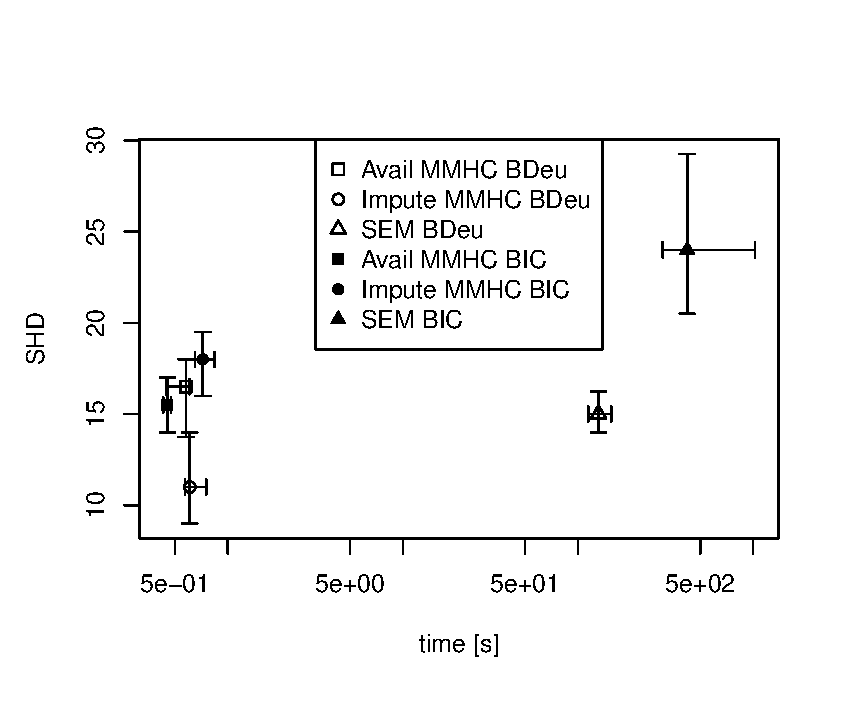
\includegraphics[width=0.75\textwidth]{figure/child_crosses_1000.eps}}
\caption{SHD vs. running time of i) available case analysis with MMHC, ii) kNN imputation followed by MMHC and iii) SEM, with both the BDeu and the BIC scoring functions, on 20 datasets with 1000 observations and $20\%$ missingness sampled from the 20-nodes Child network}\label{fig:childcrosses}
%\end{figure}

%\begin{figure}[!tpb]%figure2
\centerline{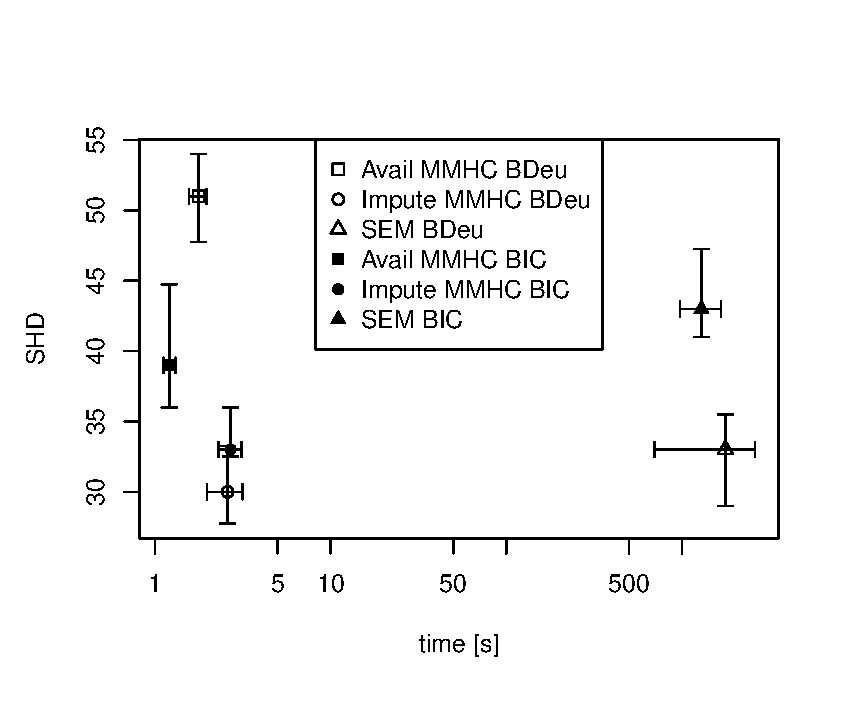
\includegraphics[width=0.75\textwidth]{figure/alarm_crosses_1000.eps}}
\caption{SHD vs. running time of i) available case analysis with MMHC, ii) kNN imputation followed by MMHC and iii) SEM, with both the BDeu and the BIC scoring functions, on 20 datasets with 1000 observations and $20\%$ missingness sampled from the 37-nodes Alarm network}\label{fig:alarmcrosses}
\end{figure}

\begin{figure}[!tpb]%figure3
\centerline{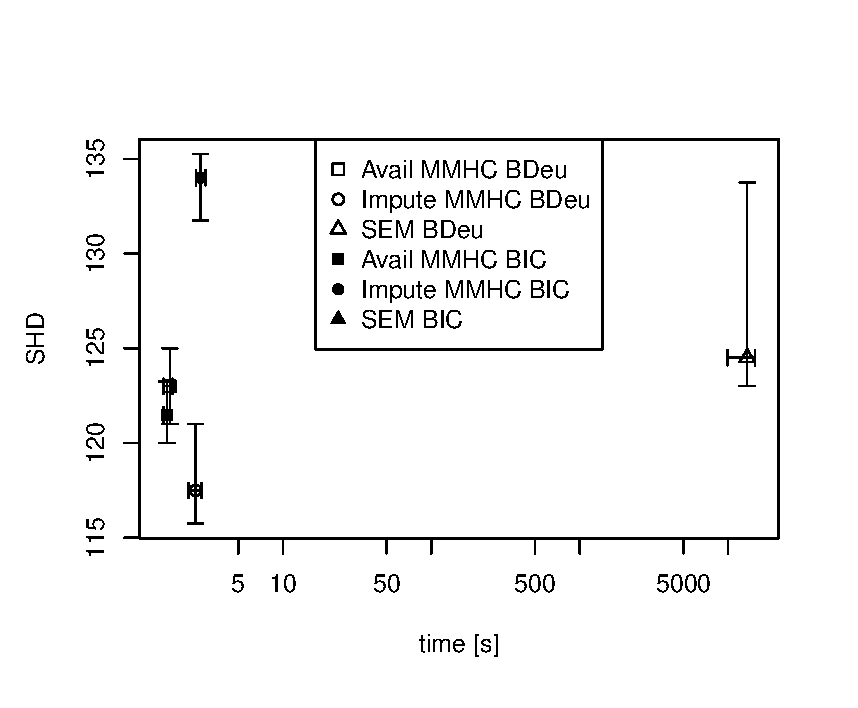
\includegraphics[width=0.75\textwidth]{figure/hepar2_crosses_1000.eps}}
\caption{SHD vs. running time of i) available case analysis with MMHC, ii) kNN imputation followed by MMHC and iii) SEM, with both the BDeu and the BIC scoring functions, on 20 datasets with 1000 observations and $20\%$ missingness sampled from the 70-nodes Hepar2 network}\label{fig:hepar2crosses}
\end{figure}

In this Section we show the results obtained by MMHC on available cases, MMHC on imputed data and SEM, with the BDeu and BIC scoring functions. Our testbed is composed by three networks available in the literature, Child (20 nodes), Alarm (37 nodes) and Hepar2 (70 nodes). For each network we consider 20 datasets of 1000 observations each, with 20\% missingness. The results for the three networks are reported, respectively, in Figures \ref{fig:childcrosses}, \ref{fig:alarmcrosses} and \ref{fig:hepar2crosses}. The datasets have been generated using our package. All the numerical parameters are set at their default value, and no prior knowledge of the network is assumed (e.g. layering).

Each plot shows the distributions of both the Structural Hamming Distance (SHD, the distance in terms of edges, on the vertical axis) from the original network, and the time needed to obtain to learn the network (in seconds, on the horizontal axis).

For all the three networks the overall best results are obtained using MMHC with BDeu after dataset imputation. MMHC converges in few seconds even for the large Hepar2 network; conversely, SEM takes from few minutes up to few hours, often with worse results. SEM paired with BIC failed to converge in 24 hours for all the 20 datasets.

\subsubsection{Parameter learning}
Parameter learning is the operation that learns the conditional probabilities entailed by a network,
given the data and the structure of the network. In \Rpackage{bnstruct} this is done by \Rmethod{learn.network}
performing a Maximum-A-Posteriori (MAP) estimate of the parameters. It is possible to choose if using the raw
or the impute dataset (\Rfunarg{use.imputed.data} parameter), and to configure the
Equivalent Sample Size (\Rfunarg{ess} parameter).

In case of using bootstrap samples, \Rmethod{learn.network} will not perform parameter learning.

\Rpackage{bnstruct} also provides the \Rmethod{learn.params} method for this task alone.

The package also provides a method for learning the parameters from a dataset with missing values using the 
Expectation-Maximization algorithm. Instructions to do so are provided in section \ref{sec:infengine}.

% \subsection{Reading a network from a file}
% Other than starting from a dataset, it is also possible to read a network from a file, formatted in a specific way
% in order to describe the structure and the parameters of the network. Several of such formats exist; we provide methods
% for two of the most widely adopted ones, the \texttt{dsc} and the \texttt{bif} format. The method names are, respectively,
% \Rmethod{read.dsc} and \Rmethod{read.bif}. These methods return a full \Robject{BN} object.
% 
% <<readfromfile,eval=FALSE>>=
% net <- read.dsc("path/to/network.dsc")
% plot(net)
% @

\section{Using a network}
Once a network is created, it can be used. Here we briefly mention some of the basic methods provided in order to
manipulate a network and access its components.

First of all, it is surely of interest to obtain the structure of a network. The \Rpackage{bnstruct} package
provides the \Rmethod{dag()} and \Rmethod{wpdag()} methods in order to access the structure of 
a network learnt without and with bootstrap (respectively).
\begin{knitrout}
\definecolor{shadecolor}{rgb}{0.969, 0.969, 0.969}\color{fgcolor}\begin{kframe}
\begin{alltt}
\hlstd{> }\hlkwd{dag}\hlstd{(net)}
\hlstd{> }\hlkwd{wpdag}\hlstd{(net)}
\end{alltt}
\end{kframe}
\end{knitrout}

Then we may want to retrieve the parameters, using the \Rmethod{cpts()} method.
\begin{knitrout}
\definecolor{shadecolor}{rgb}{0.969, 0.969, 0.969}\color{fgcolor}\begin{kframe}
\begin{alltt}
\hlstd{> }\hlkwd{cpts}\hlstd{(net)}
\end{alltt}
\end{kframe}
\end{knitrout}

Another common operation that we may want to perform is displaying the network, or printing its main informations, using the
\Rmethod{plot()}, \Rmethod{print()} and \Rmethod{show()} methods. Note that the \Rmethod{plot()} method is flexible enough to allow 
some custom settings such as the choice of the colors of the nodes, and, more importantly, some threshold settings 
for the networks learnt with bootstrap. As default, the DAG of a network is selected for plotting, if available,
otherwise the WPDAG is used. In case of presence of both the DAG and the WPDAG, in order to specify the latter as
structure to be plotted, the \Rfunarg{plot.wpdag} logical parameter is provided. As usual, more details are available
in the inline documentation of the method.
\begin{knitrout}
\definecolor{shadecolor}{rgb}{0.969, 0.969, 0.969}\color{fgcolor}\begin{kframe}
\begin{alltt}
\hlstd{> }\hlkwd{plot}\hlstd{(net)} \hlcom{# regular DAG}
\hlstd{> }\hlkwd{plot}\hlstd{(net,} \hlkwc{plot.wpdag}\hlstd{=T)} \hlcom{# wpdag}
\end{alltt}
\end{kframe}
\end{knitrout}

As it is for \Robject{BNDataset}s, we have several equivalent options to print a network.
\begin{knitrout}
\definecolor{shadecolor}{rgb}{0.969, 0.969, 0.969}\color{fgcolor}\begin{kframe}
\begin{alltt}
\hlstd{> }\hlcom{# TFAE}
\hlstd{> }\hlkwd{print}\hlstd{(net)}
\hlstd{> }\hlkwd{show}\hlstd{(net)}
\hlstd{> }\hlstd{net}
\end{alltt}
\end{kframe}
\end{knitrout}

For large biological networks it might be convenient to use some external specific tool for visualization.
We provide the \Rfunarg{write.xgmml} method to export a network in the \texttt{XGMML} format, that can be
then used for example with Cytoscape.
\begin{knitrout}
\definecolor{shadecolor}{rgb}{0.969, 0.969, 0.969}\color{fgcolor}\begin{kframe}
\begin{alltt}
\hlstd{> }\hlkwd{write.xgmml}\hlstd{(net)}
\end{alltt}
\end{kframe}
\end{knitrout}


\subsection{Inference}\label{sec:infengine}
Inference is performed in \Rpackage{bnstruct} using an \Robject{InferenceEngine} object. An \Robject{InferenceEngine}
is created directly from a network.
\begin{knitrout}
\definecolor{shadecolor}{rgb}{0.969, 0.969, 0.969}\color{fgcolor}\begin{kframe}
\begin{alltt}
\hlstd{> }\hlstd{dataset} \hlkwb{<-} \hlkwd{child}\hlstd{()}
\hlstd{> }\hlstd{net}     \hlkwb{<-} \hlkwd{learn.network}\hlstd{(dataset)}
\hlstd{> }\hlstd{engine}  \hlkwb{<-} \hlkwd{InferenceEngine}\hlstd{(net)}
\end{alltt}
\end{kframe}
\end{knitrout}

Optionally, a list of observations can be provided to the \Robject{InferenceEngine}, at its creation or later on.
The list of observations is a list of two vector, one for the observed variables
(variable indices or names can be provided, not necessarily in order - better is to list them in order of observation),
and one for the observed values for the corresponding variables. In case of multiple observations of the same variable, the last one (the most recent one) is considered.

\begin{knitrout}
\definecolor{shadecolor}{rgb}{0.969, 0.969, 0.969}\color{fgcolor}\begin{kframe}
\begin{alltt}
\hlstd{> }\hlstd{dataset} \hlkwb{<-} \hlkwd{child}\hlstd{()}
\hlstd{> }\hlstd{net}     \hlkwb{<-} \hlkwd{learn.network}\hlstd{(dataset)}
\hlstd{> }
\hlstd{> }\hlcom{# suppose we have observed variable 1 taking value 2}
\hlstd{> }\hlcom{# and variable 4 taking value 1:}
\hlstd{> }\hlstd{obs} \hlkwb{<-} \hlkwd{list}\hlstd{(}\hlstr{"observed.vars"} \hlstd{=} \hlkwd{c}\hlstd{(}\hlnum{1}\hlstd{,}\hlnum{4}\hlstd{),}
\hlstd{+ }            \hlstr{"observed.vals"} \hlstd{=} \hlkwd{c}\hlstd{(}\hlnum{2}\hlstd{,}\hlnum{1}\hlstd{))}
\hlstd{> }
\hlstd{> }\hlcom{# the following are equivalent:}
\hlstd{> }\hlstd{engine}  \hlkwb{<-} \hlkwd{InferenceEngine}\hlstd{(net, obs)}
\hlstd{> }
\hlstd{> }\hlcom{# and}
\hlstd{> }\hlstd{engine}  \hlkwb{<-} \hlkwd{InferenceEngine}\hlstd{(net)}
\hlstd{> }\hlkwd{observations}\hlstd{(engine)} \hlkwb{<-} \hlstd{obs}
\end{alltt}
\end{kframe}
\end{knitrout}

The \Robject{InferenceEngine} class provides methods for belief propagation, that is, updating
the conditional probabilities according to observed values, and for the Expectation-Maximization (EM) algorithm
(\cite{dempster1977maximum}), which learns the parameters of a network from a dataset with missing values trying
at the same time to guess the missing values.

Belief propagation can be done using the \Rmethod{belief.propagation} method. It takes an \Robject{InferenceEngine}
and an optional list of observations. If no observations are provided, the engine will use the ones it already contains.
The \Rmethod{belief.propagation} method returns an \Robject{InferenceEngine} with an \Rmethod{updated.bn}
updated network.
\begin{knitrout}
\definecolor{shadecolor}{rgb}{0.969, 0.969, 0.969}\color{fgcolor}\begin{kframe}
\begin{alltt}
\hlstd{> }\hlstd{obs} \hlkwb{<-} \hlkwd{list}\hlstd{(}\hlstr{"observed.vars"} \hlstd{=} \hlkwd{c}\hlstd{(}\hlnum{1}\hlstd{,}\hlnum{4}\hlstd{),}
\hlstd{+ }            \hlstr{"observed.vals"} \hlstd{=} \hlkwd{c}\hlstd{(}\hlnum{2}\hlstd{,}\hlnum{1}\hlstd{))}
\hlstd{> }\hlstd{engine}  \hlkwb{<-} \hlkwd{InferenceEngine}\hlstd{(net)}
\hlstd{> }\hlstd{engine}  \hlkwb{<-} \hlkwd{belief.propagation}\hlstd{(engine, obs)}
\hlstd{> }\hlstd{new.net} \hlkwb{<-} \hlkwd{updated.bn}\hlstd{(engine)}
\end{alltt}
\end{kframe}
\end{knitrout}

The EM algorithm is instead performed by the \Rmethod{em} method. Its arguments are an \Robject{InferenceEngine}
and a \Robject{BNDataset} (optionally: a convergence \Rfunarg{threshold}, the Equivalent Sample Size \Rfunarg{ess} and the maximum number of iterations \Rfunarg{max.em.iterations}),
and it returns a list consisting in an updated \Robject{InferenceEngine} and an updated \Robject{BNDataset}.

\begin{knitrout}
\definecolor{shadecolor}{rgb}{0.969, 0.969, 0.969}\color{fgcolor}\begin{kframe}
\begin{alltt}
\hlstd{> }\hlstd{dataset} \hlkwb{<-} \hlkwd{child}\hlstd{()}
\hlstd{> }\hlstd{net}     \hlkwb{<-} \hlkwd{learn.network}\hlstd{(dataset)}
\hlstd{> }\hlstd{engine}  \hlkwb{<-} \hlkwd{InferenceEngine}\hlstd{(net)}
\hlstd{> }\hlstd{results} \hlkwb{<-} \hlkwd{em}\hlstd{(engine, dataset)}
\hlstd{> }\hlstd{updated.engine}  \hlkwb{<-} \hlstd{results}\hlopt{$}\hlstd{InferenceEngine}
\hlstd{> }\hlstd{updated.dataset} \hlkwb{<-} \hlstd{results}\hlopt{$}\hlstd{BNDataset}
\end{alltt}
\end{kframe}
\end{knitrout}


\section{Two small but complete examples}
Here we show two small but complete examples, in order to highlight how the package can provide significant results
with few instructions.

First we show how some different learning setups perform on the \texttt{Child} dataset. We compare the default
\texttt{mmhc-BDeu} pair on available case analysis (raw data with missing values) and on imputed data, and
the \texttt{sem-BDeu} pair.

\begin{knitrout}
\definecolor{shadecolor}{rgb}{0.969, 0.969, 0.969}\color{fgcolor}\begin{kframe}
\begin{alltt}
\hlstd{> }\hlstd{dataset} \hlkwb{<-} \hlkwd{child}\hlstd{()}
\hlstd{> }
\hlstd{> }\hlcom{# learning with available cases analysis, MMHC, BDeu}
\hlstd{> }\hlstd{net} \hlkwb{<-} \hlkwd{learn.network}\hlstd{(dataset)}
\end{alltt}


{\ttfamily\noindent\itshape\color{messagecolor}{bnstruct :: learning the structure using MMHC ...\\bnstruct :: learning using MMHC completed.\\bnstruct :: learning network parameters ... \\bnstruct :: parameter learning done.}}\begin{alltt}
\hlstd{> }\hlkwd{plot}\hlstd{(net)}
\end{alltt}
\end{kframe}
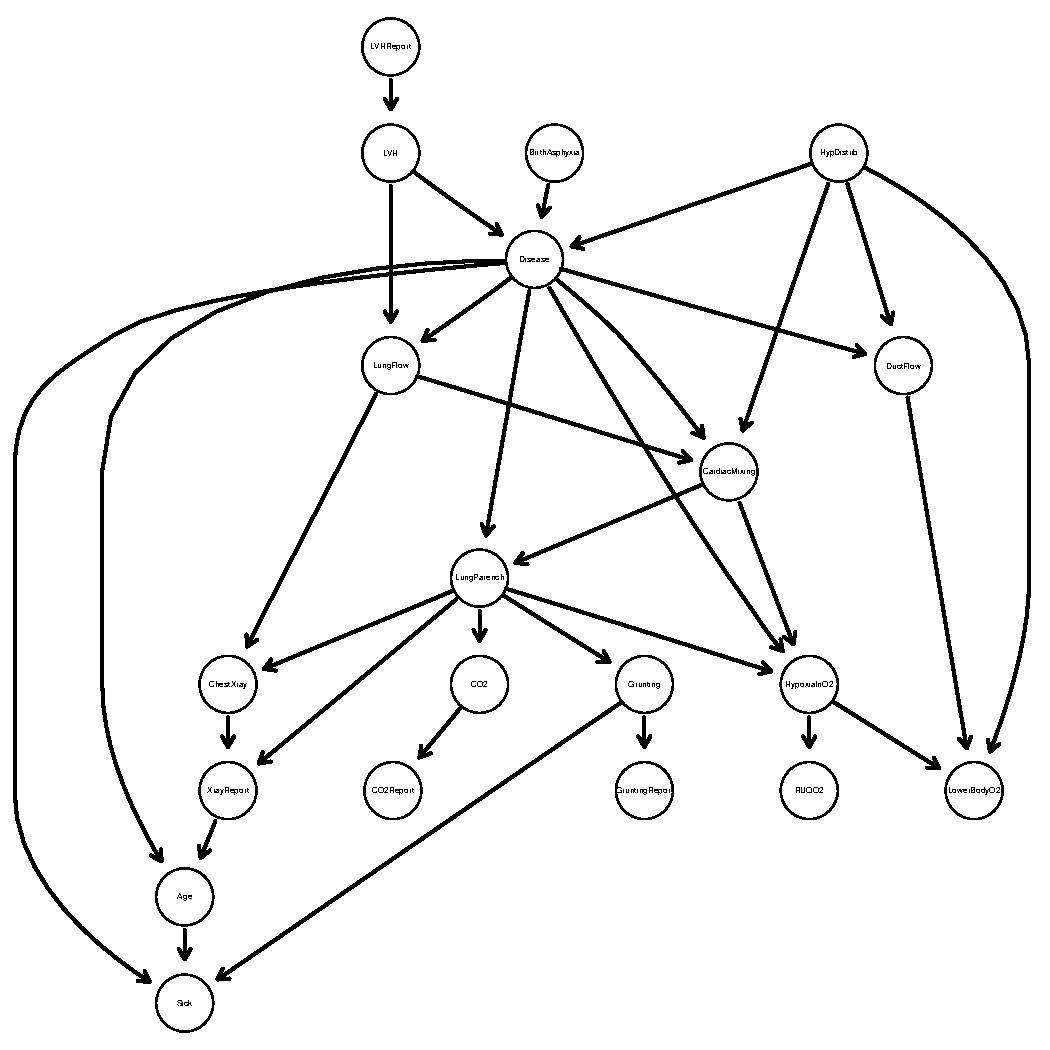
\includegraphics[width=\maxwidth]{figure/childtest-1} 
\begin{kframe}\begin{alltt}
\hlstd{> }\hlcom{# learning with imputed data, MMHC, BDeu}
\hlstd{> }\hlstd{imp.dataset} \hlkwb{<-} \hlkwd{impute}\hlstd{(dataset)}
\end{alltt}


{\ttfamily\noindent\itshape\color{messagecolor}{bnstruct :: performing imputation ...\\bnstruct :: imputation finished.}}\begin{alltt}
\hlstd{> }\hlstd{net} \hlkwb{<-} \hlkwd{learn.network}\hlstd{(imp.dataset,} \hlkwc{use.imputed.data} \hlstd{=} \hlnum{TRUE}\hlstd{)}
\end{alltt}


{\ttfamily\noindent\itshape\color{messagecolor}{bnstruct :: learning the structure using MMHC ...\\bnstruct :: learning using MMHC completed.\\bnstruct :: learning network parameters ... \\bnstruct :: parameter learning done.}}\begin{alltt}
\hlstd{> }\hlkwd{plot}\hlstd{(net)}
\end{alltt}
\end{kframe}
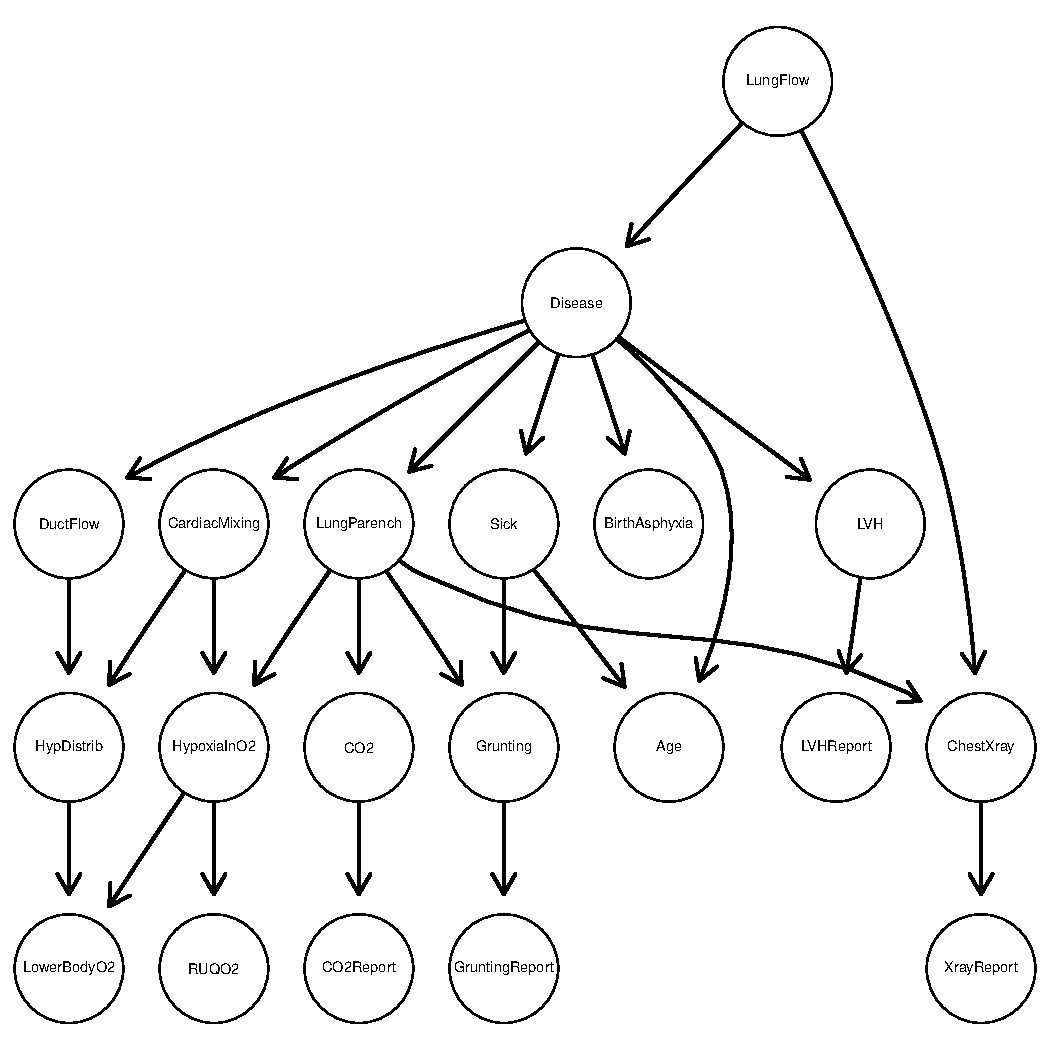
\includegraphics[width=\maxwidth]{figure/childtest-2} 
\begin{kframe}\begin{alltt}
\hlstd{> }\hlcom{# SEM, BDeu using previous network as starting point}
\hlstd{> }\hlstd{net} \hlkwb{<-} \hlkwd{learn.network}\hlstd{(dataset,} \hlkwc{algo} \hlstd{=} \hlstr{"sem"}\hlstd{,}
\hlstd{+ }                     \hlkwc{scoring.func} \hlstd{=} \hlstr{"BDeu"}\hlstd{,}
\hlstd{+ }                     \hlkwc{initial.network} \hlstd{= net,}
\hlstd{+ }                     \hlkwc{struct.threshold} \hlstd{=} \hlnum{10}\hlstd{,}
\hlstd{+ }                     \hlkwc{param.threshold} \hlstd{=} \hlnum{0.001}\hlstd{)}
\end{alltt}


{\ttfamily\noindent\itshape\color{messagecolor}{bnstruct :: learning the structure using SEM ...\\... bnstruct :: starting EM algorithm ...\\... ... bnstruct :: learning network parameters ... \\... ... bnstruct :: parameter learning done.\\... ... bnstruct :: learning network parameters ... \\... ... bnstruct :: parameter learning done.\\... bnstruct :: EM algorithm completed.\\... bnstruct :: learning the structure using MMHC ...\\... bnstruct :: learning using MMHC completed.\\... bnstruct :: learning network parameters ... \\... bnstruct :: parameter learning done.\\... bnstruct :: starting EM algorithm ...\\... ... bnstruct :: learning network parameters ... \\... ... bnstruct :: parameter learning done.\\... ... bnstruct :: learning network parameters ... \\... ... bnstruct :: parameter learning done.\\... ... bnstruct :: learning network parameters ... \\... ... bnstruct :: parameter learning done.\\... ... bnstruct :: learning network parameters ... \\... ... bnstruct :: parameter learning done.\\... bnstruct :: EM algorithm completed.\\... bnstruct :: learning the structure using MMHC ...\\... bnstruct :: learning using MMHC completed.\\... bnstruct :: learning network parameters ... \\... bnstruct :: parameter learning done.\\bnstruct :: learning using SEM completed.\\bnstruct :: learning network parameters ... \\bnstruct :: parameter learning done.}}\begin{alltt}
\hlstd{> }\hlkwd{plot}\hlstd{(net)}
\end{alltt}
\end{kframe}
\includegraphics[width=\maxwidth]{figure/childtest-3} 
\begin{kframe}\begin{alltt}
\hlstd{> }\hlcom{# we update the probabilities with EM from the raw dataset,}
\hlstd{> }\hlcom{# starting from the first network}
\hlstd{> }\hlstd{engine}  \hlkwb{<-} \hlkwd{InferenceEngine}\hlstd{(net)}
\hlstd{> }\hlstd{results} \hlkwb{<-} \hlkwd{em}\hlstd{(engine, dataset)}
\end{alltt}


{\ttfamily\noindent\itshape\color{messagecolor}{bnstruct :: starting EM algorithm ...\\... bnstruct :: learning network parameters ... \\... bnstruct :: parameter learning done.\\... bnstruct :: learning network parameters ... \\... bnstruct :: parameter learning done.\\... bnstruct :: learning network parameters ... \\... bnstruct :: parameter learning done.\\... bnstruct :: learning network parameters ... \\... bnstruct :: parameter learning done.\\bnstruct :: EM algorithm completed.}}\begin{alltt}
\hlstd{> }\hlstd{updated.engine}  \hlkwb{<-} \hlstd{results}\hlopt{$}\hlstd{InferenceEngine}
\hlstd{> }\hlstd{updated.dataset} \hlkwb{<-} \hlstd{results}\hlopt{$}\hlstd{BNDataset}
\end{alltt}
\end{kframe}
\end{knitrout}

The second example is about learning with bootstrap. This time we use the \texttt{Asia} dataset.

\begin{knitrout}
\definecolor{shadecolor}{rgb}{0.969, 0.969, 0.969}\color{fgcolor}\begin{kframe}
\begin{alltt}
\hlstd{> }\hlstd{dataset} \hlkwb{<-} \hlkwd{asia}\hlstd{()}
\hlstd{> }\hlstd{dataset} \hlkwb{<-} \hlkwd{bootstrap}\hlstd{(dataset)}
\end{alltt}


{\ttfamily\noindent\itshape\color{messagecolor}{bnstruct :: Generating bootstrap samples ...\\bnstruct :: Bootstrap samples generated.}}\begin{alltt}
\hlstd{> }\hlstd{net} \hlkwb{<-} \hlkwd{learn.network}\hlstd{(dataset,} \hlkwc{bootstrap} \hlstd{=} \hlnum{TRUE}\hlstd{)}
\end{alltt}


{\ttfamily\noindent\itshape\color{messagecolor}{bnstruct :: learning the structure using MMHC ...\\bnstruct :: learning using MMHC completed.}}\begin{alltt}
\hlstd{> }\hlkwd{plot}\hlstd{(net)}
\end{alltt}
\end{kframe}
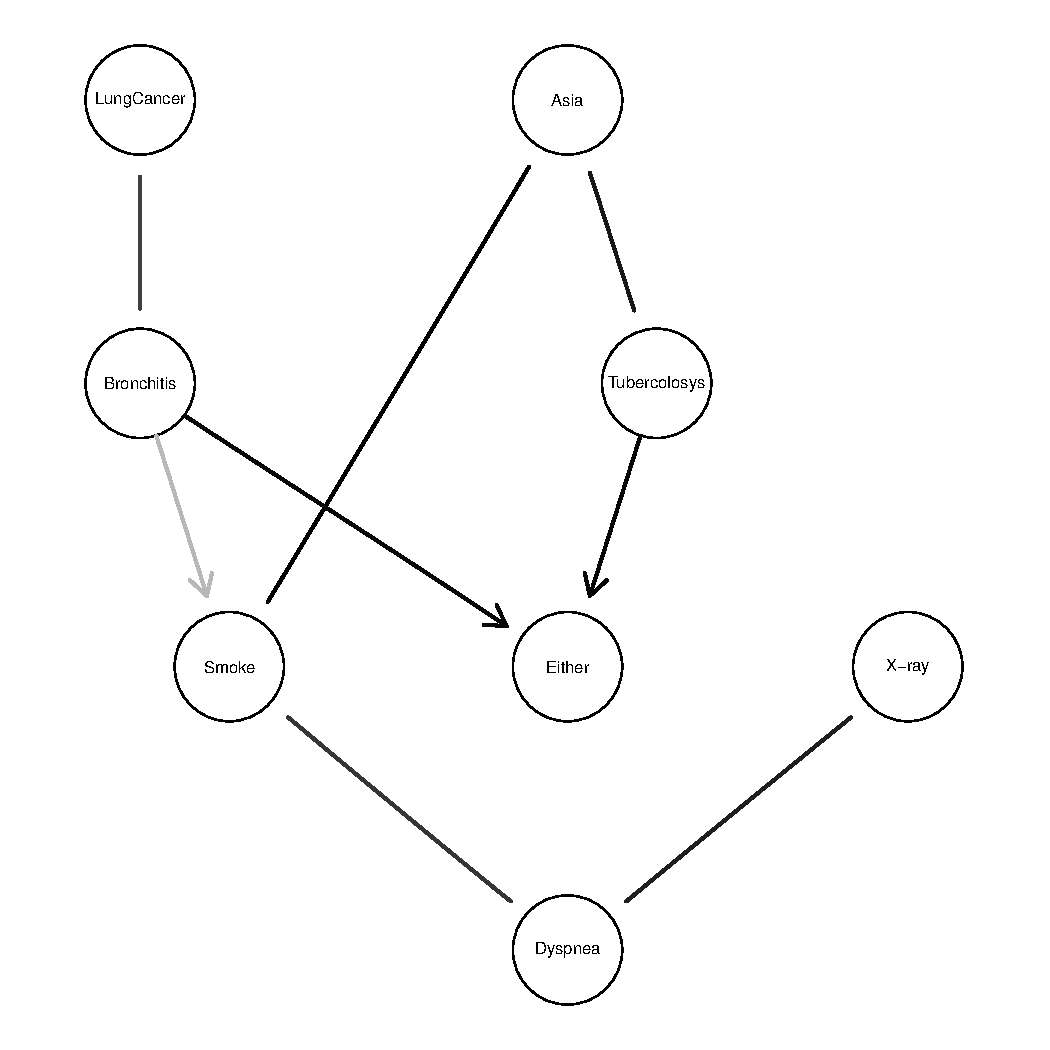
\includegraphics[width=\maxwidth]{figure/asiatest-1} 

\end{knitrout}

% -----------------------------------------------------
% 
% 
% \section{Inference in networks}
% \subsection{Belief Propagation}
% The \Rpackage{bnstruct} package provides a tool to perform belief propagation using a junction tree.
% This tool is the \Robject{InferenceEngine} object.
% It contains a copy of a network, an updated network, the adjacency matrix of the junction tree computed
% starting from the original network, the list of cliques of variables that form the nodes of the junction tree
% and the list of joint probability tables for the cliques composing the junction tree.
% 
% An \Robject{InferenceEngine} can be built from a network: in this case, the junction tree is immediately constructed.
% %Alternatively, one can use the \Rmethod{build.junction.tree} method.
% <<infeng1, eval=FALSE>>=
% dataset <- asia() # or any other way to create a custom BNDataset
% net     <- BN(dataset)
% inf.eng <- InferenceEngine(net)
% @
% % # equivalent to
% % inf.eng <- InferenceEngine()
% % bn(inf.eng) <- net
% % build.junction.tree(inf.eng, dag(net))
% % @
% 
% Belief propagation over the junction tree can be then performed using the \Rmethod{belief.propagation} method.
% <<belprop1, eval=FALSE>>=
% dataset <- asia() # or any other way to create a custom BNDataset
% net     <- BN(dataset)
% inf.eng <- InferenceEngine(net)
% inf.eng <- belief.propagation(inf.eng)
% @
% 
% Belief propagation can be fed with a list of observations. This can be done in two ways: as parameters in the method,
% or inserting them directly into the inference engine. Note that the two options are mutually exclusive, in the sense that
% the list of observations given as parameter replaces (in the whole \Robject{InferenceEngine} object returned)
% the observations contained in the engine. Furthermore, if a list of observations contains multiple observations
% of the same variable, only the last one is considered.
% <<belprop2, eval=FALSE>>=
% dataset <- asia() # or any other way to create a custom BNDataset
% net     <- BN(dataset)
% net     <- learn.structure(net, dataset)
% net     <- learn.params(net, dataset)
% inf.eng <- InferenceEngine(net)
% inf.eng <- belief.propagation(inf.eng,
%                               observed.vars = c("Asia","X-ray"),
%                               observed.vals = c(1,1))
% print(updated.bn(inf.eng))
% # is equivalent to
% observations(inf.eng) <- list(c("Asia","X-ray"), c(1,1))
% inf.eng <- belief.propagation(inf.eng)
% plot(updated.bn(inf.eng))
% @
% 
% \subsection{The Expectation-Maximization algorithm}
% Package \Rpackage{bnstruct} can also use an \Robject{InferenceEngine} and a \Robject{BNDataset} to perform
% the Expectation-Maximization algorithm to estimate the parameters of the network.
% It suffices to use the \Rmethod{em} method, that returns an \Robject{InferenceEngine} containing
% an updated network with the newly estimated conditional probability tables.
% 
% It is possible to control the algorithm by specifying the \Rfunarg{threshold} parameter, that specifies a threshold
% for the convergence of the algorithm.
% <<em1,eval=FALSE>>=
% dataset <- child() # or any other way to create a custom BNDataset
% net     <- BN(dataset)
% net     <- learn.structure(net, dataset)
% net     <- learn.params(net, dataset)
% inf.eng <- InferenceEngine(net)
% inf.eng <- em(inf.eng, dataset)
% print(updated.bn(inf.eng))
% @
% 
% \subsection{The Structural EM algorithm}
% We provide an implementation of the Structural Expectation-Maximization algorithm
% (\citet{friedman1997learning,friedman1998bayesian}),
% in order to learn both the structure and the parameters of a network in case of a dataset containing missing values.
% The method provided is \Rmethod{sem}. It accepts as parameters an \Robject{InferenceEngine} and a \Robject{BNDataset}.
% Also this method can be controlled with thresholds for the structure learning and the parameter learning steps, namely
% \Rfunarg{struct.threshold} and \Rfunarg{param.threshold}.
% 
% The method accepts also all of the parameters available for the structure learning method (see section \ref{sec:structurelearning}).
% However, the method is designed in order to follow as much as possible the settings of the original learning, whenever possible.
% For example, it is strongly recommended to adopt the same scoring function used in the learning of the network structure.
% If the network has been first learnt using \Rpackage{bnstruct}, the method will take care of that;
% in case of network read from a file, this is left to the user.
% 
% <<sem1,eval=FALSE>>=
% dataset <- child() # or any other way to create a custom BNDataset
% net     <- BN(dataset)
% net     <- learn.structure(net, dataset)
% net     <- learn.params(net, dataset)
% inf.eng <- InferenceEngine(net)
% inf.eng <- sem(inf.eng, dataset)
% plot(updated.bn(inf.eng))
% @
% 
% 
% \section{Other utilities}
% \subsection{Sample data}
% We provide also methods for generating a sample of data, or a complete dataset.
% 
% The two methods for this purpose are the \Rmethod{sample.row} and \Rmethod{sample.dataset}, that generate, respectively,
% a vector of values and a \Robject{BNDataset} object. Both the methods accept as first argument a \Robject{BN} or an
% \Robject{InferenceEngine} object. To generate a \Robject{BNDataset} with \Rmethod{sample.dataset} one should also provide the
% number of observations to sample, via the \Rfunarg{n} parameter.
% 
% <<sample,eval=FALSE>>=
% net <- BN(...)
% eng <- InferenceEngine(net)
% sample.row(net)
% sample.row(eng)
% sample.dataset(net,1000)
% sample.dataset(eng,10000)
% @


\bibliographystyle{plainnat}
\bibliography{bibtex}

\end{document}

% end
